\subsubsection{Двухуровневая архитектура}

Принцип работы двухуровневой архитектуры взаимодействия клиент-сервер заключается в том, что обработка запроса происходит на одной машине без использования сторонних ресурсов. Двухуровневая архитектура проще, так как все запросы обслуживаются одним сервером, из-за этого она более надежна но предъявляет повышенные требования к производительности сервера.

\begin{figure}[h!]
	\centering
	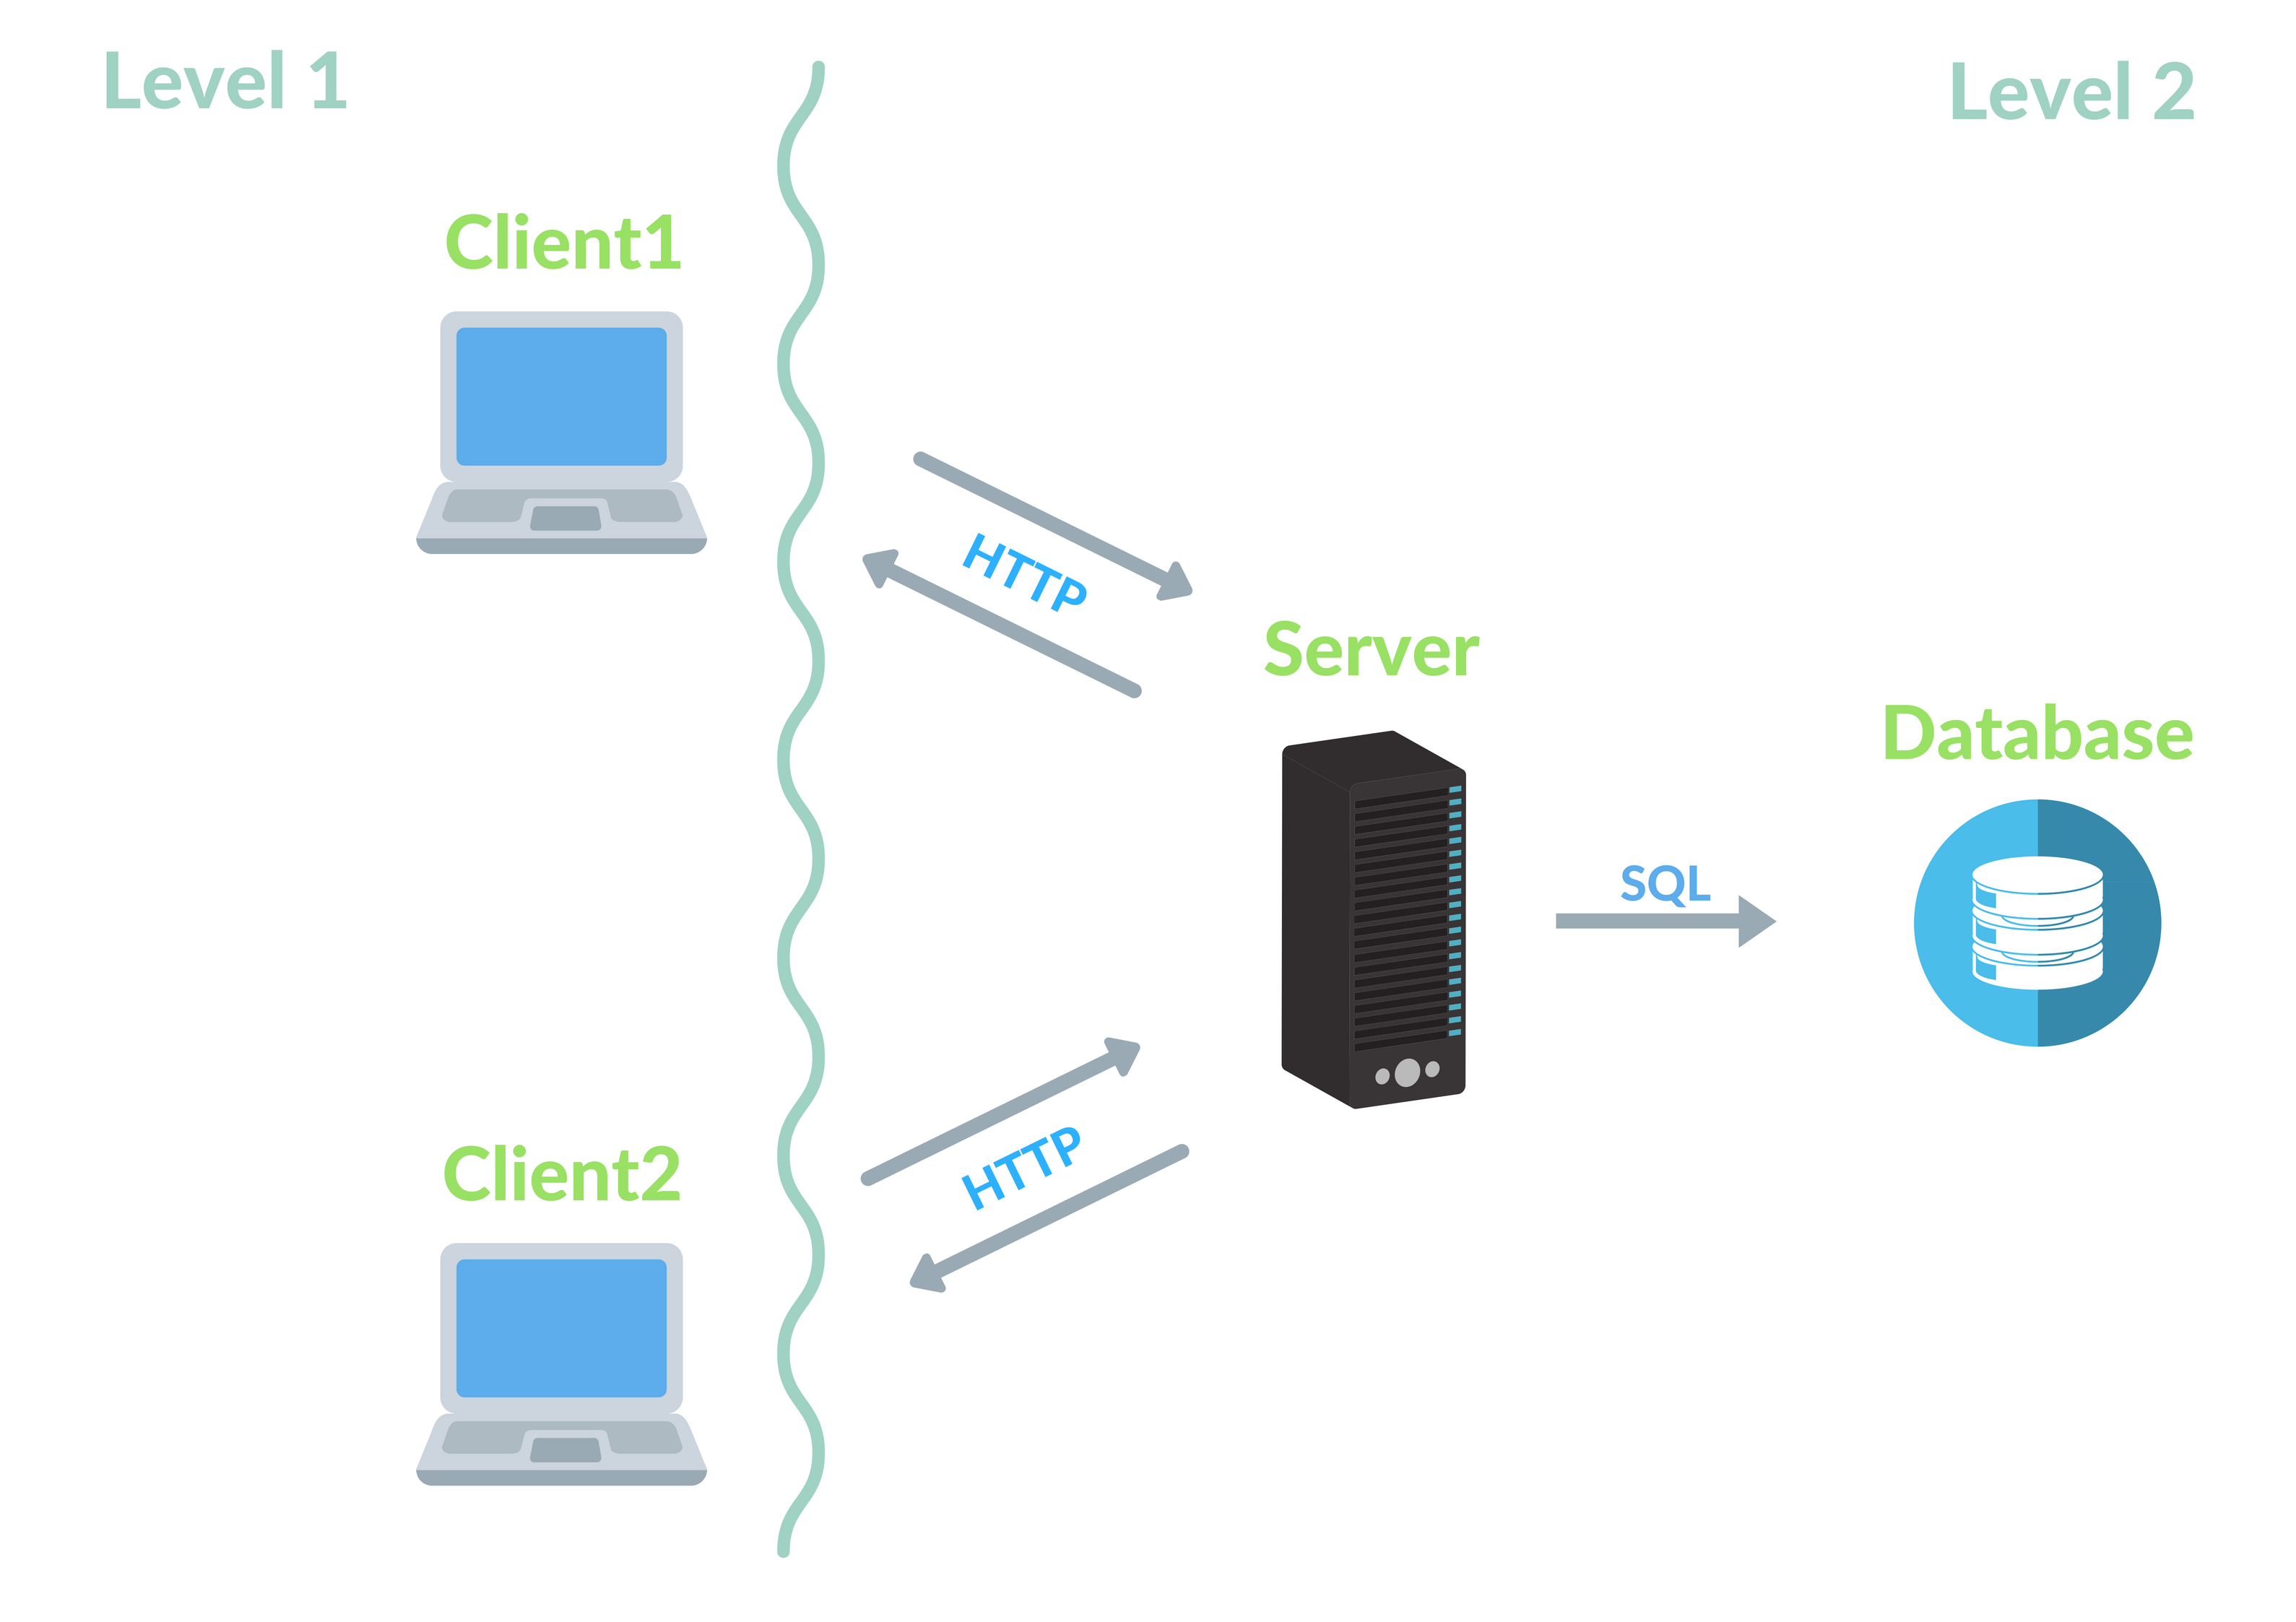
\includegraphics[scale=0.12]{2arch.png}
	\caption{Схема двухуровневой архитектуры}
	\clearpage
\end{figure}

Здесь четко видно, что есть два клиента на первом уровне, который позволяет им сделать запрос, и есть сервер, который обрабатывает запросы клиентов.